% Section 4: the dissection. Sources: FINDINGS s16-s20, s24, s25; CLAIMS B1-B8, D5, D6, E13, E16-E18, F9, G7; Gaps conflicts 1-2.
% One sentence per line; each result sentence names its FINDINGS section (s##) and CLAIMS row in its trailing comment.
\section{Dissection}
\label{sec:dissection}

This section asks which parts of OGC's VQ carry its lead over C3DGS's own: the metric, the Lloyd algorithm around it, and how many codewords it uses. % Am17 b, d; s19, s20
Only Section~\ref{sec:gram-trace} is a pre-registered test; the rest is descriptive or exploratory, as labelled. % Am17 d; CLAIMS group B

\subsection{The Gram metric against its trace}
\label{sec:gram-trace}

P2, the BD-PSNR of \code{ogc\_gram} against \code{ogc\_scalar}, isolates the metric: both rows run OGC's own Lloyd, one with the per-splat $16\times16$ Gram matrix and one with its trace, $\operatorname{tr}(G_i)/16\cdot I$. % Am17 b, d
In OGC's own Lloyd the Gram metric beat its trace at equal rate on all seven gate scenes, with $\bar P_2 = 0.1874$ dB against $2\,\mathrm{SE}_{\mathrm{noise}} = 0.0003$ dB (pre-registered; E5's verdict, Section~\ref{sec:replication}). % s19 "The verdict"; B1
Per scene P2 ran from 0.1000 dB on truck to 0.3205 dB on bonsai (Table~\ref{tab:t1}). % s19 secondaries table; B1
$\mathrm{SE}_{\mathrm{noise}}$ is seed noise at $j = 0$ only; under $\mathrm{SD}_{\mathrm{pool}}/\sqrt{n}$, the standard error that matches one curve per scene, $\bar P_2$ lay 790.14 standard errors above zero, so criterion 3 held under either convention (analysis only). % s25; B1
As for P1, this is a replication on our estimate of OGC's metric (Section~\ref{sec:setup}). % Am17 b; A12

\subsection{From C3DGS's VQ to OGC's, step by step}
\label{sec:steps}

Between C3DGS's VQ and OGC's lie three steps, each a pair of rows in the same processes: OGC's Lloyd with the identity metric against C3DGS's VQ, the trace weight against the identity, and the Gram metric against its trace (P2). % Am17 b; s19
Both other steps were positive on every scene, in BD-PSNR and at $j = 0$: \code{ogc\_scalar} minus \code{ogc\_plain} had a paired mean of $+0.0613$ dB ($\mathrm{SE}_{\mathrm{noise}}$ 0.000125) and \code{ogc\_plain} minus \code{c3dgs} $+0.2167$ dB ($\mathrm{SE}_{\mathrm{noise}}$ 0.003220) (descriptive, pre-registered secondaries without bars). % s19 secondaries; B3
The mean BD-PSNR over the seven scenes was 0.1185 dB for the identity metric against C3DGS's VQ, 0.0520 dB for the trace weight against the identity, and 0.1874 dB for the Gram metric against its trace (exploratory, not pre-registered). % s19 "Exploratory"; B2
On the development scenes (E6 part (a), descriptive) the identity step, \code{ogc\_plain} against \code{c3dgs}, was negative on flowers ($-0.013664$ dB) and treehill ($-0.077859$ dB) and positive on train ($+0.057308$ dB), so its sign on the gate scenes does not carry over. % s23 "The predictions", d; G7
These are three separate BD values, each over its own pair's shared byte range, so they do not add: they sum to 0.3579 dB against P1's 0.3558 dB (Fig.~\ref{fig:f2}). % s19 "Exploratory"; B2
As a ratio of mean BD-PSNRs the Gram step is 52.7\% of P1. % s19 "Exploratory"; B2
That share must not be read as \emph{the} metric's share: on train, the development scene, the same step was 45.9\% of the $j = 0$ difference through OGC's Lloyd, and 65.4\% of a post-hoc chain through GN-VQ's code, and the three figures measure different paths on different scenes. % s17; s18; B4, B6; CLAIMS conflict 1

\begin{figure}[t]
\centering
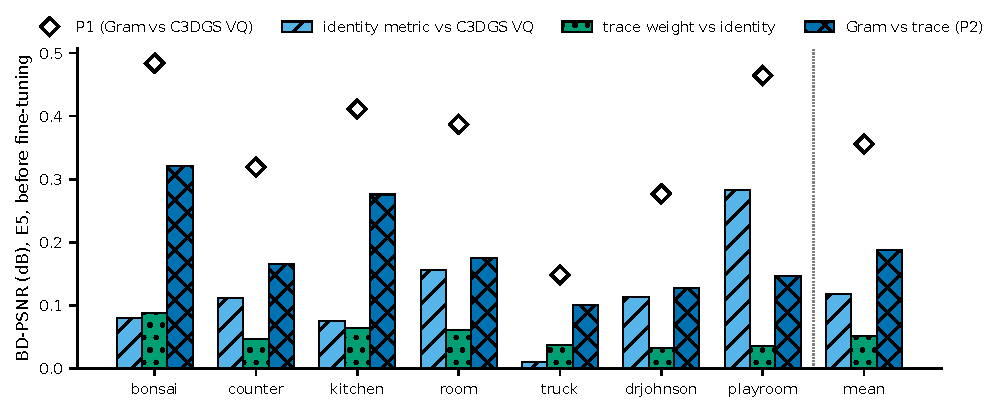
\includegraphics[width=\linewidth]{f2_p1_decomposition.pdf}
\caption{P1's steps per gate scene, E5 before fine-tuning (BD-PSNR over E5's seed-0 curves), stacked from the bottom: OGC's Lloyd with the identity metric against C3DGS's VQ, the trace weight against the identity, and the Gram metric against its trace (P2). The diamond is P1; on the mean it carries $\pm1$ standard error, $\mathrm{SD}_{\mathrm{pool}}/\sqrt{n}$, smaller than the marker. Each step is a BD value over its own pair's shared byte range, so the top of a stack is the steps' sum, not P1: over the seven scenes the steps' means sum to 0.3579 dB against P1's 0.3558 dB, and per scene the two differ by a few thousandths of a dB. Exploratory except P1 and P2.} % s19 "Exploratory"; s25; B2, A2
\label{fig:f2}
\end{figure}

\subsection{Codebook use}
\label{sec:codebook}

OGC's three rows used all 4,096 codewords in every process of every scene, while C3DGS's own VQ used 935 to 3,360, that is 22.8\% to 82.0\% of its codebook (pre-registered secondary, no bar; Fig.~\ref{fig:f5}). % s20 "Codewords used"; B8
Within a process every row shares the geometry, and only the colour arrays and the colour indices differ between rows. % s20 "Per-array bytes"; B8
Of OGC's extra bytes over C3DGS's at $j = 0$, 85.9\% to 95.0\% were its indices, which use the whole codebook nearly uniformly and so compress less. % s20 "Per-array bytes"; B8
BD-PSNR uses each row's whole \code{.npz} size, indices included. % s19 "How the numbers are computed"; A2

\begin{figure}[t]
\centering
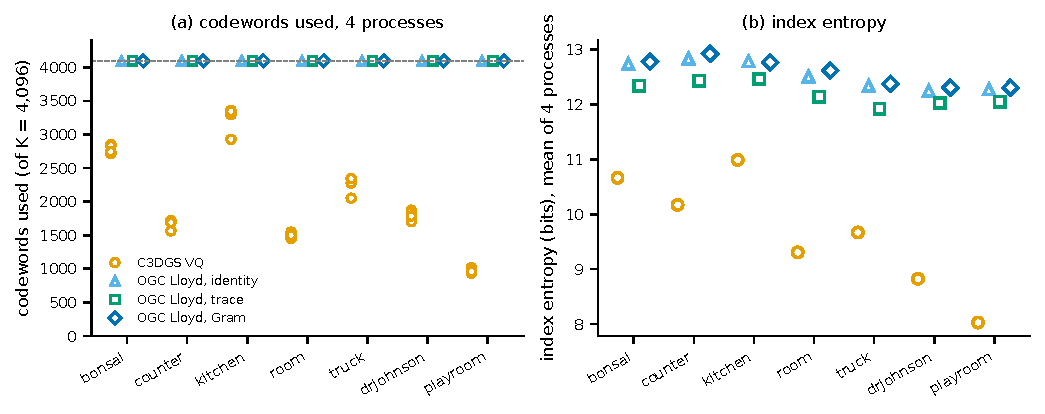
\includegraphics[width=\linewidth]{f5_codewords.pdf}
\caption{Codewords used (a) and index entropy (b) per method and gate scene, from E5's four processes per scene. OGC's three metrics use all 4,096 codewords in every process. Pre-registered secondaries, no bars.}
\label{fig:f5}
\end{figure}

\subsection{GN-VQ against OGC on the development scenes}
\label{sec:gnvq}

The project's own Gauss--Newton VQ (GN-VQ) was compared with OGC's VQ inside C3DGS only on the development scenes train and treehill, and never on a gate scene (exploratory, no verdict). % s17; Am16 b; D6
With all of OGC's algorithmic choices made in GN-VQ's code (\code{lad\_all}), GN-VQ came within 0.0013 dB of OGC's VQ on train and 0.0009 dB on treehill. % s17 "What E4q settles"; B5
The large single steps were the ones that fill empty codebook entries, reseeding ($+0.0394$ dB on train) and OGC's initial draw ($+0.0179$ dB on treehill), while each regularisation choice was worth 0.0097 dB or less, which is consistent with codebook use, rather than regularisation, being the gap between GN-VQ and OGC (exploratory, two development scenes). % s17 "What E4q settles"; B5
On train at equal rate OGC's VQ needed 14.42\% fewer bytes than GN-VQ (BD-PSNR $+0.0228$ dB), and GN-VQ's cross-validated floor was worth 0.0007 dB. % s17; s16; D6
On this evidence GN-VQ was retired from any gate before E5's code (Section~\ref{sec:setup}). % Am17 a; D6
These comparisons rest on two development scenes and do not bear on the gate scenes. % s17 "Not settled"; B5, D6

\subsection{The AC colour grid: bytes only}
\label{sec:ac-grid}

C3DGS stores the colour table through int8 quantisers whose grid, for every unfine-tuned row, is the checkpoint's own feature range, fitted to neither codebook (code reading). % s24 item 1; E16
Before fine-tuning OGC's AC codebook reached 159 to 389 grid steps beyond that grid, and 24 to 157 of its AC codebook values per process were clamped at the save, so P1 was measured with OGC's AC codebook clamped; C3DGS's AC codebook was never outside the grid (descriptive). % s24 item 2; E17
Fine-tuning re-fits the grid: OGC's AC scale grew by a factor of 1.59 to 3.16 and its \code{.npz} shrank by 10.68\% to 0.63\%, while C3DGS's AC scale changed by a factor of 0.80 to 1.13 and its \code{.npz} by $-0.31\%$ to $+1.01\%$ (descriptive; Fig.~\ref{fig:f4}). % s22 e; F9
What this records is the re-fit's effect on bytes. % s24; F9, E13
Its effect on the PSNR lead is untested, and the exploratory correlations run the wrong way for it to be the cause: across the seven scenes a larger widening of OGC's AC grid went with a smaller, not larger, fine-tuning gain difference (exploratory, $n = 7$; Spearman $\rho = -0.89$, $-0.21$ over the 28 processes and $-0.30$ after the gap-closing trend is removed). % s24 item 6; E18
E7 holds the grids, the codewords and the rest of fine-tuning fixed in turn to test this (Section~\ref{sec:ft-why}). % Am20 a; CLAIMS Gap 3

\begin{figure}[t]
\centering
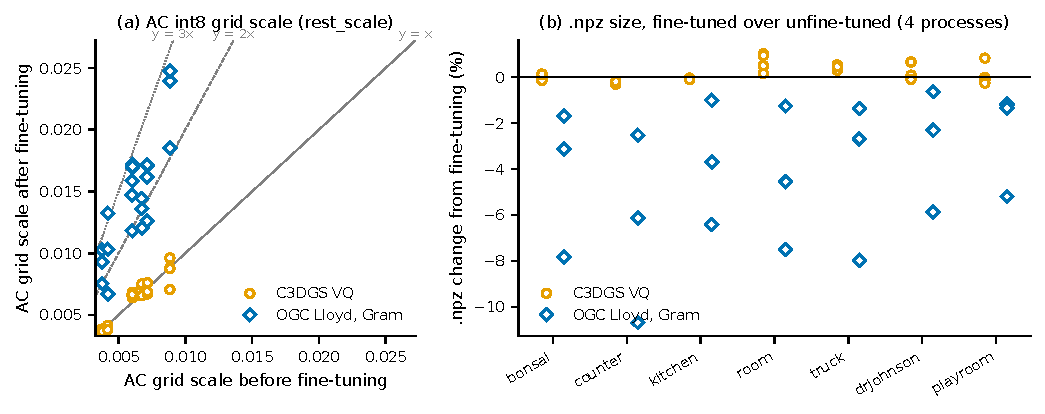
\includegraphics[width=\linewidth]{f4_ac_refit.pdf}
\caption{Fine-tuning re-fits the AC colour grid (E6 part (b), the seven gate scenes; descriptive). AC: the SH coefficients of degrees 1--3 (\code{features\_rest}). One point is one process of one scene (four per scene: $j = -1, 0, +1$ with seed 0 and $j = 0$ with seed 1), for C3DGS's VQ and for OGC's Gram-metric VQ. (a) The AC int8 grid's scale (\code{rest\_scale} of the quantizer at the save) after fine-tuning against before, with the lines $y = x$, $2x$ and $3x$. (b) The \code{.npz} size change from fine-tuning, per scene.} % s22 e; F9
\label{fig:f4}
\end{figure}
